\chapter{Implementierung des TCP/IP Stacks}
Im Rahmen dieser Arbeit wurde ein TCP Stack für die API des AMIDAR Microprozessor entwickelt. Darüber hinaus wurde der schon vorhandene IP-Stack angepasst um die gestellten Anforderungen erfüllen zu können. Zusätzlich wurde auch die Unterstützung für DHCP hinzugefügt.

\section{Überblick}
Vor Beginn dieses Projekts verfügte die AMIDAR-Java-API über grundlegende Netzwerk Funktionen. Dazu gehört der Netzwerktreiber, ein IP-Stack mit ARP-Funktionalität und ein UDP-Stack. Neu geschrieben wurde im Rahmen dieses Projekts der multithreading-fähige TCP-Stack. Dieser wurde in die vorhandene Software integriert. Des Weiteren wurde der IP-Stack erweitert und optimiert.\\\\
Sowohl beim Senden als auch beim Empfangen von Datenpaketen greifen die einzelnen Module ineinander über. Zum Empfangen von Daten prüft der Prozess des Netzwerktreibers ob neue Ethernet-Frames vorliegen. Wenn dies der Fall ist, wird eine Funktion im IP-Stack aufgerufen, die die Ethernet-Frames überprüft. Der IP-Stack unterscheidet die Pakete zwischen ARP und IP. ARP-Anfragen werden geprüft und gegebenenfalls beantwortet. Handelt es sich bei dem Datagramm um ein IP-Paket, wird ein entsprechendes Objekt erzeugt und nach weiterer Überprüfung entweder an den UDP-Stack oder an den TCP-Stack übergeben. Die Stacks für TCP und UDP beinhalten jeweils einen Table mit den vorhandenen Verbindungen, die durch Ziel- und Quell-Port identifiziert werden können. Ihnen können gegebenenfalls die erzeugten Pakete weitergegeben werden, wo sie zwischengespeichert werden. Im Falle von UDP wird die Payload ausgelesen, wenn die \textit{receive}-Methode der UDP-Connection, von einem anderen Thread aufgerufen wird. Die TCP-Connections können jeweils in ihren eigenen Thread laufen, da eine zeitnahe Verarbeitung der angekommen Pakete nötig ist, um die Verbindung zu managen. In diesem Thread werden die angekommenen Pakete ausgewertet und die dazu entsprechenden Reaktionen berechnet und ausgeführt. \\
Wenn UDP Datenpakete versendet werden sollen, wird die \textit{send}-Methode aufgerufen, die ein UDP-Paket erzeugt und dieses an den UDP-Stack weitergibt. Der wiederum erzeugt aus dem UDP-Paket ein IP-Paket, mit dem die \textit{send} Methode des IP-Stacks aufgerufen wird. Die einen Ethernetframe erzeugt und den Sendevorgang im Netzwerktreiber startet.\\ \\
Bei dem Senden von Daten über TCP wird von der Anwendung ebenfalls die \textit{send} Methode der TCP-Connection aufgerufen. Die Daten werden dabei jedoch nicht sofort gesendet, sondern in einen Puffer zwischengespeichert, vorausgesetzt der aktuelle Status der Verbindung erlaubt das. Bei Ausführung des Threads der Verbindung werden gegebenenfalls die zu übertragenden TCP-Pakete in IP-Pakete umgewandelt und analog wie die UDP-Pakete versendet. 


\begin{figure}[h]
	\centering
	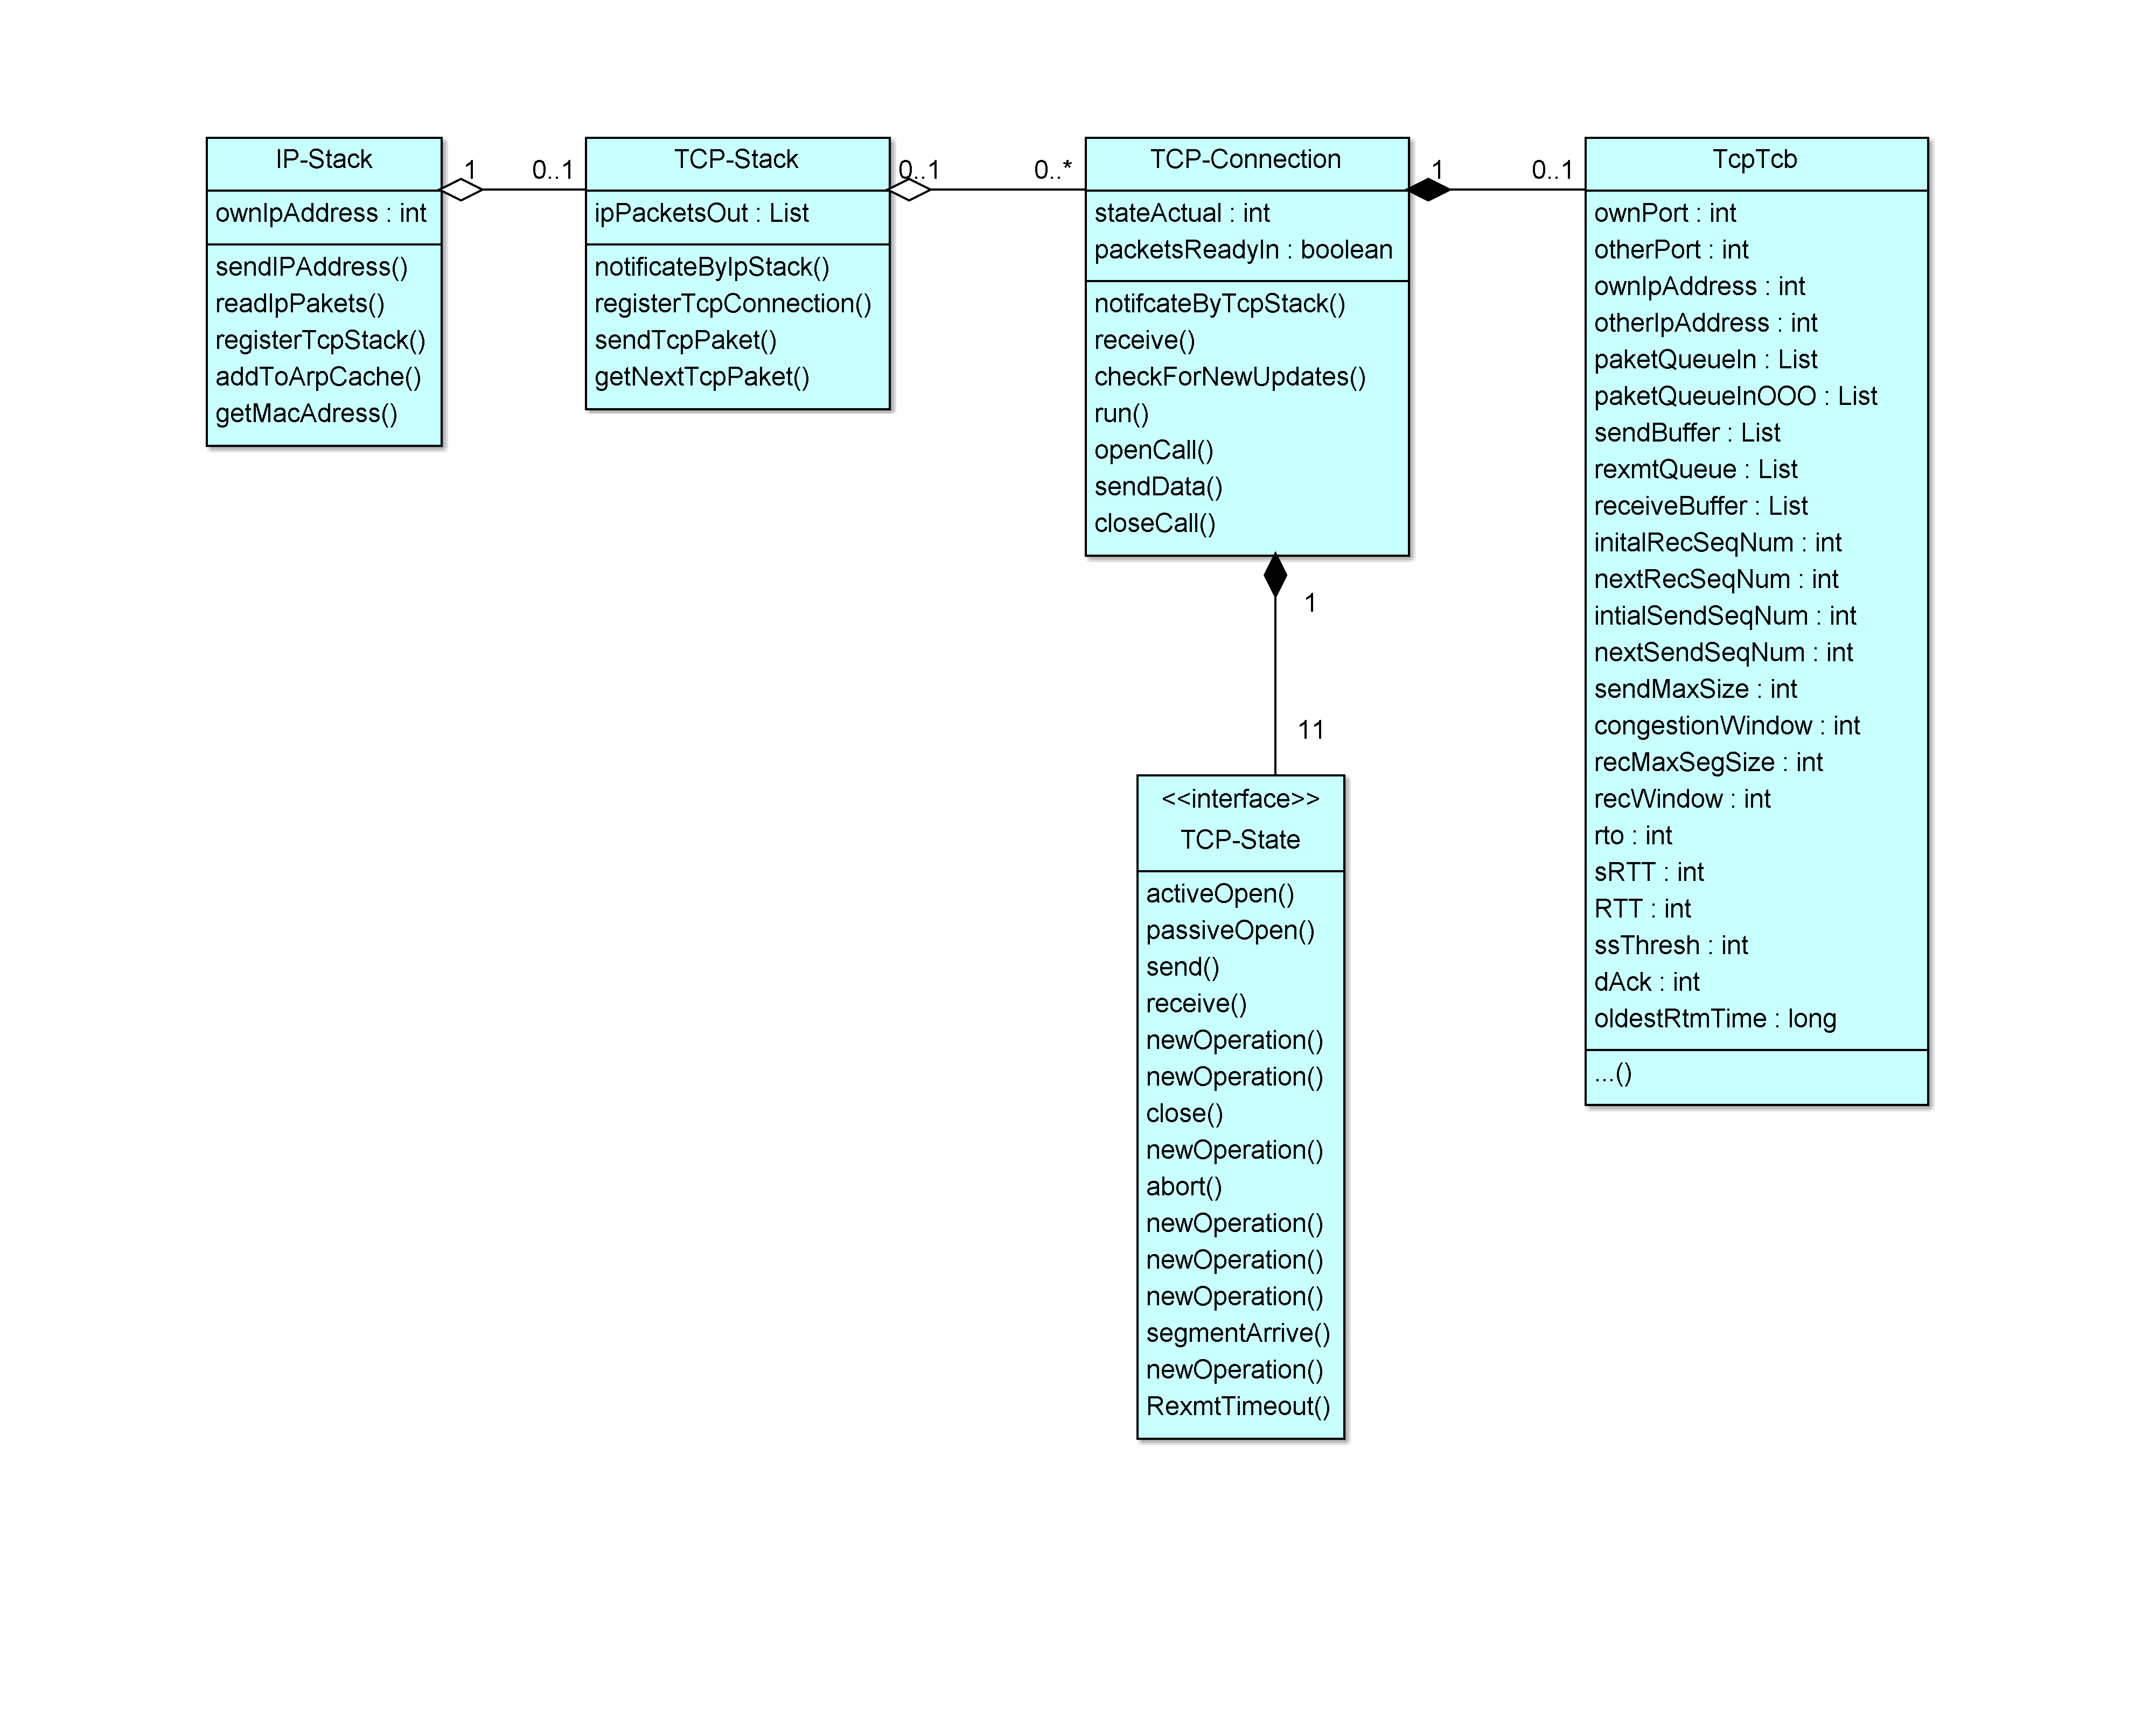
\includegraphics[width=1\textwidth]{Graphics/TCPStack.png}
	\caption{Auszug Klassendiagramm TCP/IP}		
\end{figure}


\section{IP Stack}
Der IP-Stack erfüllt mehrere Funktionen, die für eine zuverlässige Netzwerkkommunikation benötigt werden. Dazu gehört das Senden und Empfangen von IP-Pakten, ebenso wie die Unterstützung der ARP Funktionalitäten.

\subsection{IP Paket}
Für die Repräsentation von IP-Paketen wird die Klasse \textit{IpPacket} genutzt. Diese enthält die Daten des Pakets in einem Array. Neben Methoden, welche die einzelnen Felder des Header zurückgeben, gibt es Konstruktoren, die als Parameter TCP-, UDP- oder Ethernet-Pakete entgegennehmen. Des weiteren gibt es Methoden zur Berechnung der Checksumme und der Umwandlung von String Repräsentationen von IP Adressen zu Integer-Werten.  

\subsection{Empfangen von IP Paketen}

Die Methode \textit{readIpPakets} des IP-Stacks wird vom Netzwerktreiber Thread aufgerufen. In dieser werden in einer Schleife die angekommenen Ethernet-Pakete eingelesen und die IP-Pakete dazu erzeugt. Dabei werden im Zweifelsfall Teile von fragmentierten Paketen zwischengespeichert, bis diese vollständig sind. \\\\
Bei den so erzeugten IP-Paketen wird das darüber liegende Protokoll ausgelesen.\\\\
Damit UDP- und TCP-Pakete zugestellt werden können, müssen die jeweiligen Stacks im IP-Stack registriert werden. Nach der Registrierung können angekommene  Pakete dem jeweiligen Stack zugeordnet werden. Dafür implementieren beide Stacks die Funktion \textit{notificateByIpStack} der eine Liste mit angekommenen UDP-Paketen übergeben wird. 

\subsubsection{Fragmentierung}

IP-Pakete können während der Übertragung fragmentiert werden, um über Netzwerke mit einer zu niedrigen maximalen Segmentgröße übertragen zu werden. Diese werden vom Empfänger defragmentiert. \\\\
Fragmentierte Pakete können nach dem Erzeugen erkannt werden, indem das entsprechende Flag ausgelesen wird. Das Flag gibt nicht explizit an, dass dieses Paket ein Teil eines größeren fragmentierten Pakets ist, sondern dass sie ein Teil eines fragmentierten Pakets ist und weitere Paket Fragmente folgen. Das bedeutet, dass das letzte Fragment eines Pakets nicht das Flag gesetzt hat. Dieses kann man daran erkennen, dass der Fragment-Offset ungleich Null ist.\\
Der IP-Stack enthält eine Liste von fragmentierte Paketen, die Listen mit jeweils zusammengehörigen Fragmenten enthalten. Wann immer ein Paket ankommt, bei dem die {}"More Fragments"{} Flag gesetzt ist oder der Data-Offset ungleich Null ist, wird geprüft, ob dieses zu einem der fragmentierten Pakete gehört, und wird in diesem Fall in eine der Listen hinzugefügt. Die Zugehörigkeit wird dabei anhand der Identification des IP Pakets geprüft. \\
Falls ein Paket ohne Flag einem anderen fragmentierten Paket zugeordnet werden kann, ist dieses das letzte Fragment des ursprünglichen IP-Pakets, mit dem das kombinierte Paket erzeugt werden kann. \\\\
Für diesen Zweck verfügt die Klasse \textit{IpPaket} über die statische Methode \textit{fuseFragmentedIpPackets}, die eine Liste von zusammengehörigen IP-Paket-Fragmenten annimmt. Diese werden auf Kompatibilität geprüft, wobei auch die Größe der kombinierten Nutzlast berechnet wird. Die Fragmente müssen neben der identischen Identifikation über die selbe Quell- und Ziel-IP-Adresse verfügen. Des Weiteren müssen die Angaben des Frame-Offsets mit der Paketlänge plausibel sein. \\
Anschließend wird ein Array der entsprechenden Länge erzeugt und die Nutzlast der Pakete anhand des Frame-Offsets zusammengesetzt. \\Danach kann der Konstruktor der IP-Paket-Klasse aufgerufen werden, wobei ihm die neu kombinierte Nutzlast übergeben wird. Das neu erzeugte Paket wird zurückgegeben und von dem IP-Stack weiterverarbeitet. 


\subsection{Senden von IP Paketen}
Der IP-Stack verfügt über die Methode \textit{sendIpPaket}, die im Normalfall von dem TCP- oder dem UDP-Stack aufgerufen wird. Diese nimmt ein übergebenes IP-Paket an und generiert daraus einen Ethernet-Frame. Daraufhin wird das Paket über das Ethernet versendet. 


\subsection{Address Resolution Protokoll (ARP)}
Das ARP-Protokoll wird verwendet, um in einem lokalen Netzwerk die IP Adressen zu den physischen MAC-Adressen aufzulösen. Ein Host kann eine ARP-Request als Broadcast verschicken, um die MAC-Adresse zu erfahren, über die die Netzwerkressource mit der IP-Adresse zu erreichen ist. \\\\
Der IP-Stack verfügt über die Möglichkeit, ankommende ARP-Pakte zu verarbeiten. Für den Fall, dass es sich bei einem ankommenden Datenpaket anstatt eines IP-Pakets um ein ARP-Paket handelt, wird geprüft, ob es sich um eine {}"Request"{} oder eine {}"Response"{} handelt. Falls es sich um eine Request handelt, wird in einer entsprechenden Antwort die eigene physische MAC-Adresse verschickt. \\\\
Beim Versenden eines IP-Pakets muss ein Ethernet-Paket erzeugt werden. Dafür wird die MAC-Adresse unter der das Ziel oder die nächste Station auf dem Weg zu diesem erreichbar ist, benötigt. Für diesen Zweck verfügt der IP-Stack über eine Hash-Map, die als ARP-Cache dient. In dem Fall, dass für die IP kein Eintrag mit MAC-Adresse vorliegt, wird eine ARP-Request gesendet und auf deren Antwort gewartet. Nachdem die ARP-Response eingetroffen ist, wird die IP-Adresse mit der MAC-Adresse verknüpft und in dem ARP-Cache gespeichert. 


 



\section{TCP}

Vor der Implementierung des TCP-Stacks wurde überprüft, ob es schon in Java implementierte TCP-Stacks gibt. Die einzige in Frage kommende Implementierung war der "{}ejlP"{}-TCP-Stack. Dieser verfügt jedoch über keinen Mechanismus für die erneute Übertragung verlorener Pakete, die von dem darüber liegenden Protokoll gewährleistet werden müsste. Aus diesem Grund wurde entschieden, eine eigene TCP-Variante zu schreiben, die keine umfassende Änderung des IP-Stacks und des Treibers erforderte.\cite{ejlP}



\subsection{TCP Stack}
Der TCP-Stack stellt den Datenaustausch zwischen den einzelnen TCP-Verbindungen und dem IP-Stack her und ist dabei in der Lage, mehrere Verbindungen parallel offen zu haben und diese einzeln zu verwalten. 
Er enthält eine Map mit allen angelegten TCP-Verbindungen. Es gibt eine Funktion, um neue TCP-Verbindungen zu registrieren. Eine der wichtigsten Methoden ist textit{notificateByIpStack}, die vom IP-Stack aufgerufen wird und eine Liste von TCP-Paketen übergibt. Der TCP Stack untersucht diese und überprüft sie anhand der Checksumme auf Korrektheit. Fehlerhafte Pakete werden aussortiert. Fehlerfreie werden abhängig von der Ziel-Port-Nummer an eine der TCP-Verbindungen übergeben oder verworfen, wenn diese keiner Verbindung zugeordnet werden können.   

\subsection{TCP Verbindung}
Die Klasse \textit{TcpConnection} verwaltet die Zustände und Datenströme einer Verbindung. Die Klasse stellt zum einen die Verbindung zu der Anwendung dar und zum anderen enthält sie den Zustandsautomaten, der die Abläufe bei dem Aufbauen und Aufrechterhalten der Verbindung managt. Des Weiteren befindet sich in dieser der Transmission-Control-Block (TCB), der nach dem Öffnen einer Verbindung die meisten für diese Verbindung spezifischen Variablen enthält.   

\subsection{TCP-Paket}
TCP-Pakete werden von einer Klasse repräsentiert, welche die Daten des Paktes in einem Array speichert, auf dessen Datenfelder mit entsprechenden Methoden gezielt zugegriffen werden kann. Außerdem gibt es Methoden zur Berechnung der Prüfsumme.


\subsubsection{Struktur Zustandsautomat}
Eine TCP-Verbindung muss auf eine Reihe von Ereignissen abhängig von der aktuellen Situation reagieren, dabei bietet sich ein Zustandsautomat an, der jeden Zustand durch eine eigene Klasse abstrahiert. Da es bei der momentan von AMIDAR unterstützen JAVA-Version 1.4 noch keine Unterstützung für Enumerationen gibt, werden die einzelnen Zustände in einem Array von \textit{TcpClass} gespeichert. \textit{TcpClass} ist dabei das Interface, das alle Statusklassen implementiert. Der aktuelle Zustand wird jeweils von der Integer-Variable \textit{actualState} angegeben, welche die Position im Zustandsarray angibt. Falls eine der zustandsabhängigen Methoden aufgerufen werden soll, wird diese auf dem Array aufgerufen, wobei \textit{actualState} als Index genutzt wird. Das von den Zustandsklassen implementierte Interface enthält folgende Methoden:
\begin{description}
\item[activeOpen:] Öffnet eine Verbindung und versucht mit dem übergebenen Port und der IP-Adresse den Drei-Wege-Handshake zu initiieren. 
\item[passiveOpen:] Öffnet eine Verbindung, auf die von anderen Geräten ein Verbindungsaufbau initiert werden kann. 
\item[send:] Schreibt übergebene Daten in den Sende-Puffer des TCP-Stacks und erzeugt gegebenenfalls ein neues TCP-Paket, welches die übergebenen Daten verschickt. 
\item[receive:] Überprüft, ob genug Daten vorhanden sind, um diese an die Anwendung zu übergeben. 
\item[close:] Signalisiert, dass alle Daten übertragen wurden und die Verbindung abgebaut werden kann. 
\item[abort:] Bricht die Verbindung ab.
\item[segmentArrive:] Untersucht und verarbeitet ein ankommendes TCP-Paket.
\item[RexmtTimeout:] Wird aufgerufen, nachdem ein Timeout für ein Paket in der \textit{Retransmit Queue} aufgetreten ist. 
\end{description}
Jede dieser Methoden gibt als Integer den nächsten Zustand zurück. \textit{Active Open}, \textit{Passive Open}, \textit{send}, \textit{receive}, \textit{close} und \textit{abort} werden durch Aufrufe der darüber liegenden Anwendung ausgelöst. \textit{Segment Arrive} wird aufgerufen, nachdem vom TCP-Stack angekommene Pakete übergeben wurden und der Thread der Verbindung ausgeführt wird. 
\textit{RexmtTimeout} wird aufgerufen, wenn der Retransmit-Timer für ein Paket ausläuft. 

\subsubsection{Neue Übertragung verlorener Pakete}
Jedes gesendete Paket wird mit einem Zeitstempel versehen und der \textit{Retransmit-Queue} hinzugefügt. Der Zeitstempel des ältesten Paket in der \textit{Retransmit-Queue}, wird als Basis genommen, um zu bestimmen, ob ein Timeout vorliegt. Die vergangene Zeit, bis ein Retransmit ausgelöst wird, wird nicht willkürlich gewählt, da so bei Verbindungen mit hoher Latenz Pakete neu versendet würden, die nicht verloren gegangen sind. Diese Zeit, RTO genannt, wird abhängig von der Round-Trip-Time (RTT) berechnet. Die Round-Trip-Time gibt die Zeit an, die vergeht, nachdem ein Paket übergeben wurde, bis das Acknowledgement für dieses Paket eingetroffen ist.  Um zu starke Schwankungen bei der RTO zu vermeiden, wird eine geglättete Round Trip Time verwendet. \\\\
$SRTT = (\alpha * SRTT) + ((1-\alpha)*RTT)$\\
$RTO = min [u, max [o, (\beta *SRTT)]]$\\\\
Der Glättungsfaktor $\alpha$ wird zwischen 0,8 und 0,9 festgelegt. $\beta$ ist ein Varianzfaktor und wird auf einen Wert zwischen 1,3 und 2,0 gesetzt.Die Variablen "{}u"{} und "{}o"{} stellen die obere und untere Grenze dar und werden beispielsweise auf eine Sekunde bzw. eine Minute gesetzt.


\subsubsection{Transmission-Control-Block(TCB)}

Der Transmission-Control-Block enthält alle für die Verbindung wichtigen Variablen, abgesehen von der Zustandsvariable.  Dazu gehören der eigene Port und der Port des Zielrechners, die eigene IP-Adresse und die der Gegenstelle. Darüber hinaus werden die Sequenznummern sowohl zum Empfangen als auch zum Senden gespeichert.  Des Weiteren finden sich dort alle Variablen, die zur "{}Congestion-Contol"{} benötigt werden.  


\subsubsection{Zustände im Detail}
Sofern nicht anders beschrieben, löst ein Timeout eines Pakets eine neue Übertragung von diesem aus, wobei es am Ende der \textit{Retransmission-Queue}, mit einem neuen Zeitstempel gespeichert wird. Wenn ein Paket nach dem 5. Timeout noch nicht angekommen sein sollte, wird davon ausgegangen, dass keine nutzbare Verbindung zum Host mehr existiert und die Verbindung wird abgebrochen. 
Bei allen weiteren in den jeweiligen Zuständen nicht näher beschriebenen Aktionen wird eine \textit{IOException} geworfen.

\begin{description}
%\subsub
\item[CLOSED:]
In diesen Zustand wird bei einem \textit{activOpen} ein Verbindungsaufbau gestartet. Dafür wird die initiale Sequenznummer zufällig generiert und ein SYN-Paket erzeugt. Anschließend wird die \textit{SendUnacknowledged}-Nummer auf den Wert der initialen Sequenznummer gesetzt und der Wert für die nächste Sendesequenznummer auf die um Eins erhöhte intiale Sequenznummer gesetzt. Des Weiteren wird der nächste Zustand auf SYN-SENT gesetzt. \\
Falls die Methode \textit{passivOpen} aufgerufen wird, wird in den Zustand LISTEN gewechselt. \\
In beiden Open Methoden wird die Verbindung im TCP-Stack registriert und es wird ein Transmission-Control-Block angelegt.\\
Alle anderen Usercalls werden mit Fehlermeldungen beendet. 

\item[LISTEN:]
Im Zustand LISTEN wird auf einen Verbindungsaufbau von einem externen Host gewartet. Ein \textit{activeOpen}-Usercall kann auch in diesem Zustand noch ausgeführt werden, mit demselben Ablauf wie im Zustand CLOSED. Bei einem \textit{receive} Aufruf können noch keine Daten zurückgegeben werden, da keine aktive Verbindung aufgebaut ist. Der \textit{Receive}-Usercall wird jedoch zwischengespeichert. 
Die Calls \textit{close} und \textit{abort} löschen den TCB und geben den Zustand CLOSED zurück.
Bei eintreffenden Paketen wird geprüft, ob es sich um ein SYN-Paket handelt. In diesem Fall wird die Initiale Sequenznummer berechnet und ein SYN-ACK Paket in die Paket-out-Queue abgelegt. Daraufhin geht die Verbindung in den Zustand SYN-RECEIVED über. Alle anderen eintreffenden Pakete deuten auf eine Fehlfunktion der Verbindung der Gegenstelle hin und werden mit einen RST-Paket beantwortet. 


\item[SYN-RECEIVED:]
In diesem Zustand werden Aufrufe der \textit{send}- und \textit{receive}- calls zwischengespeichert, um in einem späteren Zustand ausgewertet zu werden. 
Bei Ausführung eines \textit{close}-Aufrufs wird geprüft, ob der Sendepuffer leer ist. Wenn das nicht der Fall ist, verbleibt die Verbindung im aktuellen Zustand. Andernfalls wird ein FIN-Paket gesendet, um das Ende der Verbindung einzuleiten. 
Wird die "{}abort"{}-Funktion aufgerufen, wird ein RST-Paket gesendet, der TCB gelöscht und in den Zustand CLOSED zurück gegangen.\\\\
Ankommende Pakete werden nach Überprüfung der Gültigkeit anhand der Sequenznummer ausgewertet. Ist das angekommene Paket ein ACK-Paket, wird das bestätigte Paket aus der \textit{Retransmit-Queue} entfernt und in den Established Zustand gewechselt. \\ Falls ein weiteres SYN- oder ein RST-Paket ankommt, wird die Verbindung beendet. 

	
\item[SYN-SEND:]
Die Aktionen für \textit{send}, \textit{receive},\textit{ close} und \textit{abort} werden genauso gehandhabt, wie im Zustand SYN-RECEIVED.
Nach dem Eintreffen von gültigen SYN-ACK Paketen wird in den Zustand ESTABLISHED gewechselt. Wenn ein eintreffendes Paket nur ein SYN enthält wird der Zustand SYN-RECEIVED zurück gegeben und ein SYN-ACK-Paket gesendet. Bei einem RST-Paket wird die Verbindung abgebrochen. Alle anderen Pakete werden verworfen.   
	
\item[ESTABLISHED:]

In diesem Zustand beginnt die \textit{send} Operation mit dem Speichern der übergebenen Daten in den Sendepuffer. Anschließend wird das maximale Limit an Daten bestimmt, die noch versendet werden dürfen. Dafür wird das Minimum von \textit{Congestion Window}, und \textit{Receiver-Window} genutzt. Anschließend wird ein Datenpaket erzeugt, wobei darauf geachtet wird, das sowohl dass Limit, als auch die maximale Segment-Größe nicht überschritten wird. \\\\
Ankommende Datenpakete werden einsortiert. Entspricht die Sequenznummer des Pakets der erwarteten Sequenznummer, können die Daten des Pakets in den Empfangspuffer geschrieben werden. Ist die Sequenznummer über der erwarteten Nummer, werden die Pakete in den "{}Out-of-Order"{} Puffer zwischengespeichert. Diese werden, wenn das fehlende Paket ankommt, hinter dem neuen Paket in den Empfangspuffer einsortiert. Jedes ankommende Paket wird mit einem ACK-Paket quittiert. Dabei ist zu beachten, dass bei Paketen, die nicht in der erwarteten Reihenfolge ankommen, die Sequenznummer des erwarteten Pakets als Acknowledge-Nummer gesendet wird. Dadurch wird der Gegenseite signalisiert, dass dieses Paket möglicherweise verloren gegangen ist. Dadurch enstehen duplizierte ACKs,  die für  "{}Fast Retransmit"{} und "{} Fast Recovery"{} essentiell ist.\\\\
Des Weiteren wird das mit dem Paket mitgeschickte ACK überprüft. Entspricht die Acknowledge-Nummer der letzten nicht bestätigten gesendeten Sequenznummer, wird ein Zähler um eins hoch gesetzt um duplizierte ACKs zu erkennen. Bei einem mehr als dreimal duplizierten ACK wird ein {}"Fast Retransmit"{} durchgeführt. Dabei wird die \textit{Slow-Start-Threshold} halbiert und die Größe des \textit{Congestion-Windows} auf den Wert von diesem gesetzt. Zusätzlich wird das verlorene Paket aus der \textit{Retransmit-Queue} herausgesucht und sofort neu übertragen. Wenn ein gültiges, nicht dupliziertes ACK eintrifft, werden alle bestätigten Segmente aus der \textit{Retransmit-Queue} entfernt und das \textit{Congestion-Window} entsprechend der "{}Slow Start"{} und "{}Congestion Avoidance"{} Algorithmen erhöht. Falls das FIN-Flag bei einem gültigen Paket gesetzt ist, wird der Zustand CLOSE WAIT zurück gegeben.  \\\\
Falls es zu dem Timeout eines Pakets kommt, wird die \textit{Slow Start Threshold} ebenfalls halbiert und das \textit{Congestion-Window} auf den initialen Wert gesetzt. 

\item[FIN-WAIT-1:]

In diesem Zustand wird auf ankommende Pakete mit derselben Art reagiert wie im Zustand ESTABLISHED, mit dem Unterschied, dass nach einem ankommenden gültigen ACK-Paket in den Zustand FIN-WAIT-2 gewechselt wird. Ist zusätzlich auch das FIN-Flag gesetzt, wird in den Zustand TIME-WAIT übergegangen. Dazu kommt, dass bei duplizierten ACK-Paketen kein {}"Fast-Retransmit"{} mehr durchgeführt wird.

\item[FIN-WAIT-2:]	
Ankommende Pakete werden hier verarbeitet wie in der ESTABLISHED Phase mit dem Unterschied, dass bei einen FIN-Paket der Zustand TIME-WAIT zurückgegeben wird.


\item[CLOSE-WAIT:]

In diesem Zustand funktioniert ein \textit{send} Call genauso wie im Zustand ESTABLISHED. Bei ankommenden Segmenten werden nur noch ankommende ACK-Pakete verarbeitet, da die Gegenstelle keine Daten mehr senden wird. Nach der Ankunft von SYN- oder RST-Paketen wird die Verbindung beendet. \\
Nach einen Aufruf von \textit{close} Call wechselt die Verbindung in den Zustand LAST-ACK und sendet ein FIN-Paket.

\item[LAST-ACK:]

In diesem Zustand lösen alle Usercalls bis auf \textit{Segment Arrive} eine \textit{IOException} aus. Ankommende gültige Pakete werden daraufhin untersucht, ob diese das ACK zu dem gesendeten FIN-Paket sind. Ist dies der Fall, wird die Verbindung beendet und in den Zustand CLOSED übergegangen. Bei der Ankunft eines RST- oder SYN-Pakets wird die Verbindung abgebrochen und ebenfalls der Zustand CLOSED zurückgegeben.

\item[CLOSING:]

Der Zustand CLOSING verhält sich weitgehend identisch zum Zustand LAST-ACK, mit dem Unterschied, dass in den Zustand TIME-WAIT übergegangen wird, wenn ein ankommendes Paket das ACK für das gesendete FIN-Paket enthält.


\item[TIME-WAIT:]
In diesem Zustand ist der Verbindungsabbau abgeschlossen. Die Verbindung bleibt dennoch ein paar Minuten offen um stark verzögerte Pakete zu bestätigen. Das Eintreffen von RST- und SYN-Paketen beendet die Verbindung sofort.

\end{description}

\subsubsection{Options}
TCP-Optionen werden in einem optionalen Bereich mit variabler Länge des Headers abgelegt. Um diese zu repräsentieren, wurde eine Klasse erstellt, um den Optionsbereich des TCP-Headers abzubilden. Dafür wurde eine Methode geschrieben, um die Optioncodes in eine übersichtliche Datenstruktur zu parsen. Zusätzlich gibt es eine Methode, um Optionen in eine Datenstruktur zu überführen und daraus den Optionsblock im TCP Header zu generieren. Es wurde jedoch keine Unterstützung für konkrete Optionen implementiert.



\section{Zero Copy}
Die TCP- und IP-Pakete werden jeweils durch eine entsprechende Klasse repräsentiert. Die Objekte dieser Klasse enthalten jeweils ein Array, das Header und Nutzdaten des Pakets enthält. Beide Klassen verfügen über einen Konstruktor, der jeweils die andere der beiden Klassen als Parameter entgegennimmt. So kann beim Senden aus einem TCP-Paket ein IP-Paket erzeugt werden und beim Empfangen aus einen IP-Paket ein TCP-Paket. Dabei stellt das TCP-Paket die Nutzlast des IP-Pakets da. Um in diesem Fall lange Kopiervorgänge zu ersparen, wird es vermieden, ein neues Array anzulegen und die Daten hinein zu kopieren. Anstelle dessen wird in der TCP-Paket-Klasse im Array ein 20 Byte Puffer eingeplant, in den später der IP-Header geschrieben werden kann. Bei der Erzeugung eines IP-Pakets aus einen TCP-Paket wird das im TCP-Paket erzeugte Array weiterverwendet. Da die ersten 20 Byte leer sind, kann dort der IP Header geschrieben werden.


\section{DHCP}
Das Dynamic-Host-Control-Protocol verwendet UDP in der Transportschicht, um die Nachrichten zu senden. Bei der Implementierung muss eine Repräsentation der Pakete geschrieben werden um DHCP-Pakete verarbeiten zu können. Des Weiteren wird eine Klasse benötigt, die den Ablauf und die Kommunikation verarbeitet. 

\subsection{DHCP-Paket}
Die Klasse \textit{DHCPPacket} repräsentiet DHCP-Pakete. Diese enthält ein Integer-Array, welches die Paketdaten enthält. Es gibt Getter-Methoden, die mit Bitmaskierungen einzelne Datenfelder auslesen und deren Werte zurückgeben. Eine Schwierigkeit bei DHCP liegt darin begründet, dass die meisten wichtigen Informationen nicht in den festen Feldern, sondern in den variablen Optionsteilen abgelegt werden. Um diese auszulesen, musste ein Parser geschrieben werden, der den Optionsbereich einliest und nach dem übergebenen Optionscode sucht. Wenn dieser gefunden wird, werden anhand der folgenden Längenangaben die Optionsdaten ausgelesen. Beim Parsen muss beachtet werden, dass Optionen byteweise eingelesen werden müssen, obwohl diese als 32 Bit-Wörter vorliegen. 

\subsection{DHCP-Controller}

Der DHCP-Controller enthält den Thread, welcher den DHCP-Client steuert. Für die Ablaufsteuerung wurde ebenfalls ein kleiner Zustandsautomat implementiert. Sobald der Thread gestartet wurde, wird eine DISCOVER-Nachricht als Broadcast gesendet und in den Zustand SELECTING gewechselt. In diesem Zustand wird auf eine OFFER-Nachricht des Servers gewartet. Die DHCP-Nachrichten werden identifiziert, indem der Optionscode 53 aus dem Optionsblock ausgelesen wird. Der Datenwert dieser Option gibt die Art des DHCP-Paketes an. Sobald ein DHCP-OFFER eintrifft, wird die vorgeschlagene IP mit einer REQUEST angefragt und in den Zustand REQUESTING gewechselt. Bei dieser Anfrage wird die IP-Adresse mit dem Optionscode 50 angefragt. Anschließend wird auf die ACK-Nachricht gewartet, in welcher die IP-Adresse bestätigt wird. Anschließend muss noch mit einer ARP-Request geprüft werden, ob diese Adresse schon von einem andern Host im Netzwerk verwendet wird. 

\section{Packet Builder}

Ein Problem bei der Erzeugung der Paketobjekte war, dass jedes Mal eine Reihe von Parametern gesetzt werden muss, die bis auf wenige Fälle den selben Standardwert haben. Die müssen dennoch bei jeder Paket-Erzeugung gesetzt werden, was aufwändig und fehleranfällig ist. Um das zu vermeiden, können die Klassen für TCP- und DHCP-Pakete mit einen "{}Builder Pattern"{} erzeugt werden.  Dabei wird eine spezielle Builder-Klasse genutzt, die als Attribute die Parameter der Paket-Klasse enthält. Diese werden vorinitialisiert. Über spezielle Setter-Methoden können die Werte gesetzt werden. Diese geben als Rückgabewert das Builderobjekt zurück. Der letzte Aufruf auf das Objekt ist jeweils die \textit{build} Funktion, welche den Konstruktor der Paketklasse aufruft und dieses zurück gibt. Ein derartiger Aufruf sieht Beispielsweise wie folgt aus: 
\lstset{language=Java}
\begin{lstlisting}
new TcpPaketBuilder(tcb).setSeqNum(NextSendSeqNum)
.setAckNum(NextRecseqNum).setAck().build()
\end{lstlisting}
Das erzeugen eines TCP-Pakets ohne die Verwendung des "{}Builder Patterns"{} sieht folgender maßen aus: 

\begin{lstlisting}
new TcpPaket(payLoad,length,tcpOptions, 
connection, seqNum, ackNum, (short)winSize, flags ,urgP);
\end{lstlisting}



